\documentclass{article}

%% begin preamble

\usepackage[utf8]{inputenc}  % input encoding utf-8
\usepackage[T1]{fontenc}  % font encoding - T1

\usepackage{fullpage}  % for narrower margins
\usepackage{hyperref} % for urls 
\usepackage{booktabs} % For \toprule, \midrule and \bottomrule
\usepackage{siunitx} % Formats the units and values
\usepackage{csvsimple}  % generates table from mixed csv
\usepackage{pgfplotstable} % Generates table from numeric csv

\usepackage{minted}  % for source code highlighting
\setminted[python]
{
    frame=lines,  % sets the bounding box
    autogobble,  % gobbles up white-space
    framesep=2mm,  % frame seperation distance
    linenos  % sets line numbers
}
% Setup siunitx:
\sisetup{
  round-mode          = places, % Rounds numbers
  round-precision     = 2, % to 2 places
}

\pgfplotsset{compat=1.15}

\usepackage{multirow}
\usepackage{multicol}

\usepackage{xcolor}  % include all the contents of preamble.tex

\usepackage{pgfplots}
\pgfplotsset{compat=newest}
\usepgfplotslibrary{groupplots}

\title{\LaTeX{} 201 \\ Plots}
\author{Satyaki Sikdar}
\date{\today}

%% end preamble 

\begin{document}

\maketitle

Useful links \url{https://sourceforge.net/projects/pgfplots/}, \url{http://pgfplots.sourceforge.net/pgfplots_talk_FTUG_2012_final.pdf}

\section{Function plots}
\begin{figure}[htb]
    \centering
    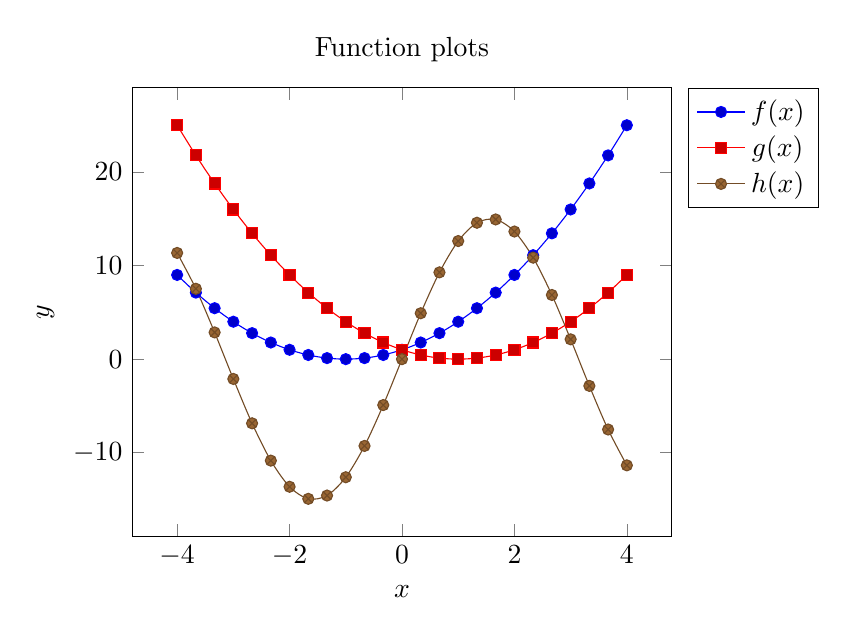
\begin{tikzpicture}
        \begin{axis}
        [
        title={Function plots},  % title of the plot
        xlabel=$x$, % x axis label
        ylabel=$y$,  % y axis label
        domain=-4:4,  % x limits
        legend pos=outer north east,  % try other directions
        smooth,  % make it a smooth plot 
        ]
             \addplot+ {x^2 + 2*x + 1};  % the + tells it to use a different style
             \addlegendentry{$f(x)$};
             
             \addplot+ {x^2 - 2*x + 1};
             \addlegendentry{$g(x)$};
             
             \addplot+ {15*sin(deg(x))};
             \addlegendentry{$h(x)$}
        \end{axis}
    \end{tikzpicture}
    \caption{Caption}
    \label{fig:func}
\end{figure}

\newpage 
\section{Scatter plots}
\begin{figure}[htb]
    \centering
    \begin{tikzpicture}
        \begin{axis}
        [
        title={Pokemon attack v. defense},  % title of the plot
        xlabel={Defense}, % x axis label
        ylabel={Attack},  % y axis label
        legend pos=outer north east,  % try other directions
        scatter,
        only marks,
        ]
        
        \addplot table
        [
        x=attack, 
        y=defense, 
        col sep=comma,
        restrict expr to domain={\coordindex}{0:200}
        ] 
        {./data/pokemon_all.csv};
        \end{axis}
    \end{tikzpicture}
    \caption{Pokemon attack v. defense for the first 200 pokemons}
    \label{fig:pokemon-attack}
\end{figure}
\newpage

\begin{tikzpicture}
	\begin{axis}[%
	xlabel = $x$,
	ylabel = $y$,
	legend pos=outer north east,
    scatter/classes={%
		a={mark=square*,blue},%
		b={mark=triangle*,red},%
		c={mark=o,draw=black}}]
	\addplot[scatter,only marks,%
		scatter src=explicit symbolic]%
	table[meta=type] {
    x     y      type
    0.1   0.15   a 
    0.45  0.27   c 
    0.02  0.17   a 
    0.06  0.1    a 
    0.9   0.5    b 
    0.5   0.3    c 
    0.85  0.52   b 
    0.12  0.05   a 
    0.73  0.45   b 
    0.53  0.25   c 
    0.76  0.5    b 
    0.55  0.32   c
	};
	
	\legend{a, b, c};
	\end{axis}
\end{tikzpicture}

\newpage 
\section{Bar plots}

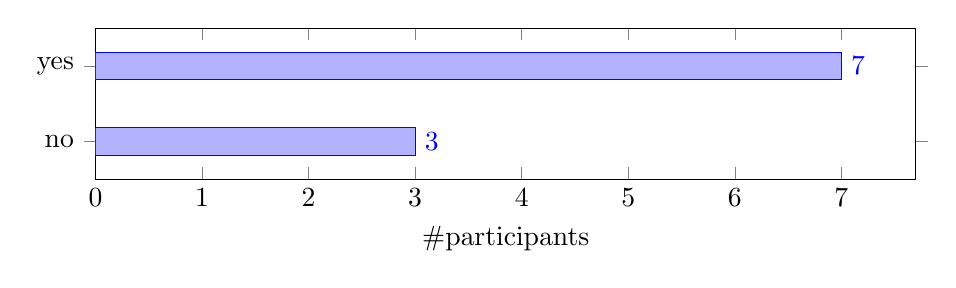
\begin{tikzpicture}
  \begin{axis}[
    xbar, 
    xmin=0,
    width=12cm, 
    height=3.5cm, 
    enlarge y limits=0.5,
    xlabel={\#participants},
    symbolic y coords={no,yes},
    ytick=data,
    nodes near coords, nodes near coords align={horizontal},
    ]
    \addplot coordinates {(3,no) (7,yes)};
  \end{axis}
\end{tikzpicture}

\newpage 
\section{Histograms}

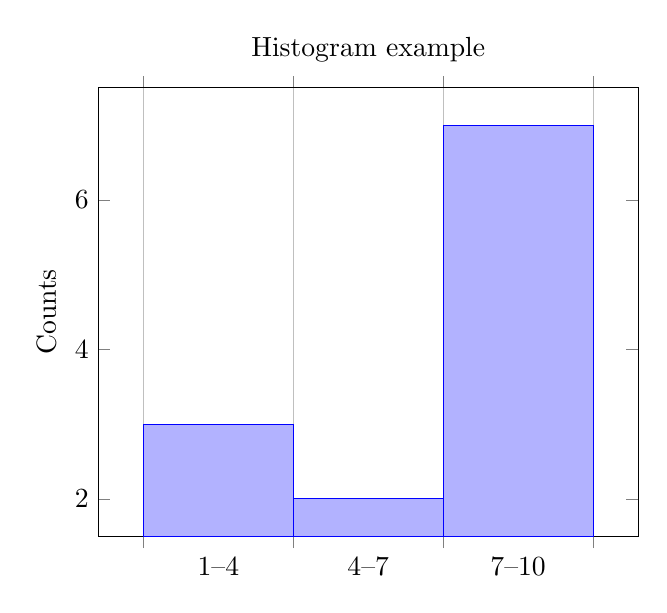
\begin{tikzpicture} 
\begin{axis}
[
  ybar interval,
  title= Histogram example,
  ylabel= Counts,
  xticklabel=
\pgfmathprintnumber\tick--\pgfmathprintnumber\nexttick
]
    \addplot+[hist={bins=3}]
        table
        [
        row sep=\\,
        y index=0
        ] 
        {
        data\\
        1\\ 2\\ 1\\ 5\\ 4\\ 10\\
        7\\ 10\\ 9\\ 8\\ 9\\ 9\\
    };
\end{axis}
\end{tikzpicture}

\newpage 
\section{Grid plots}

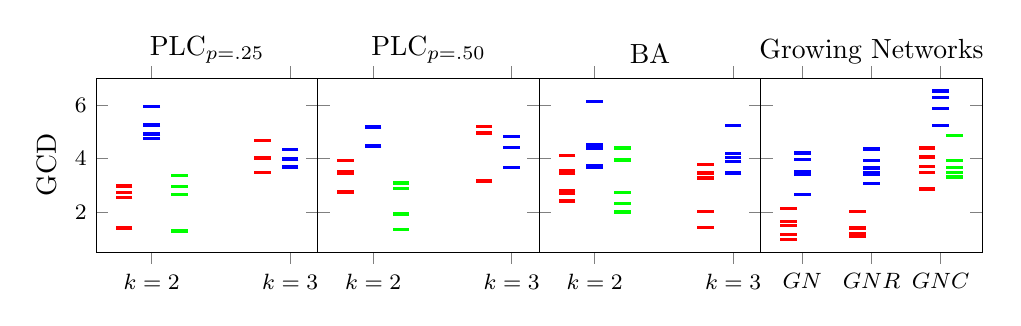
\begin{tikzpicture}

\begin{groupplot}[
    width=1.73in,
    group style={group size=4 by 1,
        horizontal sep=0pt,
        xlabels at=edge bottom,xticklabels at=edge bottom,ylabels at=edge left,yticklabels at=edge left,},
    ybar,
    every tick label/.append style={font=\footnotesize},
    ylabel near ticks,
    xlabel near ticks,
    y label style={at={(axis description cs:-0.02,.5)}},
    title style={yshift=-1.0ex,},
    %
	%xlabel={{Nodes}},
	ylabel={{GCD}},
    title={{PLC$_{p=.25}$}},
    xmax=11,
    xmin=3,
    ymin=0.5,
    ymax=7,
    ylabel near ticks,
    xtick={5, 10},
    xticklabels={$k=2$, $k=3$},
    % symbolic x coords={PSHRG, STERGM, ER},
]


\nextgroupplot[title={{PLC$_{p=.25}$}},]

% PSHRG PLC GCD p=0.25 k=2
\addplot
[
draw=none,
mark=-,
mark size=3pt,
color=red,
very thick
]
coordinates {
(4, 1.4024999999999999) +- (0, 0)
(4, 2.5316470588235296) +- (0, 0)
(4, 2.9754814814814816) +- (0, 0)
(4, 2.73540625) +- (0, 0)
};

% ER PLC GCD p=0.25 k=2
\addplot
[
draw=none,
mark=-,
mark size=3pt,
color=blue,
very thick
]
coordinates {
(5, 5.247999999999999) +- (0, 0)
(5, 5.952411764705881) +- (0, 0)
(5, 4.912148148148149) +- (0, 0)
(5, 4.7463125) +- (0, 0)
};

% STERGM PLC GCD p=0.25 k=2
\addplot
[
draw=none,
mark=-,
mark size=3pt,
color=green,
very thick
]
coordinates {
(6, 1.2925) +- (0, 0)
(6, 3.3499999999999996) +- (0, 0)
(6, 2.9400370370370372) +- (0, 0)
(6, 2.651064516129032) +- (0, 0)
};



% STERGM PLC GCD p=0.25 k=2
\addplot
[
draw=none,
mark=-,
mark size=3pt,
color=green,
very thick
]
coordinates {
(6, 1.2925) +- (0, 0)
(6, 3.3499999999999996) +- (0, 0)
(6, 2.9400370370370372) +- (0, 0)
(6, 2.651064516129032) +- (0, 0)
};

%%%% k = 3

% PSHRG PLC GCD p=0.25 k=3
\addplot
[
draw=none,
mark=-,
mark size=3pt,
color=red,
very thick
]
coordinates {
(9, 4.662166666666667) +- (0, 0)
(9, 4.0125) +- (0, 0)
(9, 3.4715454545454545) +- (0, 0)
};



% ER PLC GCD p=0.25 k=3
\addplot
[
draw=none,
mark=-,
mark size=3pt,
color=blue,
very thick
]
coordinates {
(10, 3.683833333333333) +- (0, 0)
(10, 4.3345) +- (0, 0)
(10, 3.9771818181818186) +- (0, 0)
};

% STERGM PLC GCD p=0.25 k=3
\addplot
[
draw=none,
mark=-,
mark size=3pt,
color=green,
very thick
]
coordinates {};

%%%%%%%%%% 

\nextgroupplot[title={{PLC$_{p=.50}$}},]

%%% k = 2

% PSHRG PLC GCD p=0.5 k=2
\addplot
[
draw=none,
mark=-,
mark size=3pt,
color=red,
very thick
]
coordinates {
(4, 3.510666666666667) +- (0, 0)
(4, 3.9348) +- (0, 0)
(4, 3.427666666666667) +- (0, 0)
(4, 2.75151724137931) +- (0, 0)
};


% ER PLC GCD p=0.5 k=2
\addplot
[
draw=none,
mark=-,
mark size=3pt,
color=blue,
very thick
]
coordinates {
(5, 4.472333333333334) +- (0, 0)
(5, 5.176559999999999) +- (0, 0)
(5, 5.20530303030303) +- (0, 0)
(5, 4.450068965517241) +- (0, 0)
};

% STERGM PLC GCD p=0.5 k=2
\addplot
[
draw=none,
mark=-,
mark size=3pt,
color=green,
very thick
]
coordinates {
(6, 1.335333333333333) +- (0, 0)
(6, 3.076217391304348) +- (0, 0)
(6, 2.8643636363636364) +- (0, 0)
(6, 1.9231851851851853) +- (0, 0)
};
  
%%% k = 3

% PSHRG PLC GCD p=0.5 k=3
\addplot
[
draw=none,
mark=-,
mark size=3pt,
color=red,
very thick
]
coordinates {
(9, 5.1885) +- (0, 0)
(9, 4.950222222222223) +- (0, 0)
(9, 3.1550000000000007) +- (0, 0)
};

% ER PLC GCD p=0.5 k=3
\addplot
[
draw=none,
mark=-,
mark size=3pt,
color=blue,
very thick
]
coordinates {
(10, 3.6514999999999995) +- (0, 0)
(10, 4.8245555555555555) +- (0, 0)
(10, 4.407928571428571) +- (0, 0)
};


% STERGM PLC GCD p=0.5 k=3
\addplot
[
draw=none,
mark=-,
mark size=3pt,
color=green,
very thick
]
coordinates {
};

%%%%%%%%%
\nextgroupplot[title={{BA}},]

% PSHRG BA GCD k=2
\addplot
[
draw=none,
mark=-,
mark size=3pt,
color=red,
very thick
]
coordinates {
(4, 3.5434000000000005) +- (0, 0)
(4, 2.7049333333333334) +- (0, 0)
(4, 2.4043684210526317) +- (0, 0)
(4, 4.098771428571427) +- (0, 0)
(4, 3.424913793103449) +- (0, 0)
(4, 2.8101232876712325) +- (0, 0)
};


% ER BA GCD k=2
\addplot
[
draw=none,
mark=-,
mark size=3pt,
color=blue,
very thick
]
coordinates {
(5, 4.477299999999999) +- (0, 0)
(5, 3.6488666666666663) +- (0, 0)
(5, 3.725947368421052) +- (0, 0)
(5, 6.131628571428571) +- (0, 0)
(5, 4.498362068965517) +- (0, 0)
(5, 4.377369863013699) +- (0, 0)
};


% STERGM BA GCD k=2
\addplot
[
draw=none,
mark=-,
mark size=3pt,
color=green,
very thick
]
coordinates {
(6, 2.31) +- (0, 0)
(6, 2.0104) +- (0, 0)
(6, 1.9983157894736845) +- (0, 0)
(6, 4.3880333333333335) +- (0, 0)
(6, 3.941035087719298) +- (0, 0)
(6, 2.7292916666666667) +- (0, 0)
};

%%%% k = 3

% PSHRG BA GCD k=3
\addplot
[
draw=none,
mark=-,
mark size=3pt,
color=red,
very thick
]
coordinates {
(9, 3.7803333333333335) +- (0, 0)
(9, 2.028) +- (0, 0)
(9, 1.4215) +- (0, 0)
(9, 3.453583333333333) +- (0, 0)
(9, 3.267518518518519) +- (0, 0)
};

% ER BA GCD k=3
\addplot
[
draw=none,
mark=-,
mark size=3pt,
color=blue,
very thick
]
coordinates {
(10, 4.173166666666666) +- (0, 0)
(10, 3.451) +- (0, 0)
(10, 4.035) +- (0, 0)
(10, 5.223833333333334) +- (0, 0)
(10, 3.8769629629629634) +- (0, 0)
};

% STERGM BA GCD k=3
\addplot
[
draw=none,
mark=-,
mark size=3pt,
color=green,
very thick
]
coordinates {
};

%%%%%

\nextgroupplot[title={Growing Networks},xmax=18,xmin=2,xtick={5, 10, 15},xticklabels={$GN$, $GNR$, $GNC$},]

% PSHRG GN
\addplot
[
draw=none,
mark=-,
mark size=3pt,
color=red,
very thick
]
coordinates {
(4, 1.6498000000000002) +- (0, 0)
(4, 2.125973684210527) +- (0, 0)
(4, 1.5048645833333332) +- (0, 0)
(4, 1.161725) +- (0, 0)
(4, 0.9778) +- (0, 0)
};

% ER GN
\addplot
[
draw=none,
mark=-,
mark size=3pt,
color=blue,
very thick
]
coordinates {
(5, 2.6623999999999994) +- (0, 0)
(5, 3.5102631578947374) +- (0, 0)
(5, 3.4006145833333328) +- (0, 0)
(5, 4.206975) +- (0, 0)
(5, 3.9571199999999997) +- (0, 0)
};

% STERGM GN
\addplot
[
draw=none,
mark=-,
mark size=3pt,
color=green,
very thick
]
coordinates {
};

%%%%%%%%%%%%%%%%%%%%%
%GNR
% PSHRG GNR
\addplot
[
draw=none,
mark=-,
mark size=3pt,
color=red,
very thick
]
coordinates {
(9, 1.3728) +- (0, 0)
(9, 2.0232) +- (0, 0)
(9, 1.1789193548387098) +- (0, 0)
(9, 1.3978478260869562) +- (0, 0)
(9, 1.161808510638298) +- (0, 0)
(9, 1.093035714285714) +- (0, 0)
};

% ER GNR
\addplot
[
draw=none,
mark=-,
mark size=3pt,
color=blue,
very thick
]
coordinates {
(10, 3.9163999999999994) +- (0, 0)
(10, 3.0558800000000006) +- (0, 0)
(10, 3.405725806451613) +- (0, 0)
(10, 3.6380760869565214) +- (0, 0)
(10, 3.486829787234042) +- (0, 0)
(10, 4.351464285714286) +- (0, 0)
};

% STERGM GNR
\addplot
[
draw=none,
mark=-,
mark size=3pt,
color=green,
very thick
]
coordinates {
};

%%%%%%%%%%%%%%
%GNC
% GNC PSHRG
\addplot
[
draw=none,
mark=-,
mark size=3pt,
color=red,
very thick
]
coordinates {
(14, 4.386272727272727) +- (0, 0)
(14, 2.852125) +- (0, 0)
(14, 3.4641481481481486) +- (0, 0)
(14, 4.059129032258064) +- (0, 0)
(14, 3.7106551724137935) +- (0, 0)
};

% GNC ER
\addplot
[
draw=none,
mark=-,
mark size=3pt,
color=blue,
very thick
]
coordinates {
(15, 6.539363636363637) +- (0, 0)
(15, 5.227625) +- (0, 0)
(15, 5.857407407407407) +- (0, 0)
(15, 6.289451612903226) +- (0, 0)
(15, 6.51851724137931) +- (0, 0)
};

% GNC STERGM
\addplot
[
draw=none,
mark=-,
mark size=3pt,
color=green,
very thick
]
coordinates {
(16, 4.855363636363635) +- (0, 0)
(16, 3.658) +- (0, 0)
(16, 3.4717916666666664) +- (0, 0)
(16, 3.914322580645161) +- (0, 0)
(16, 3.307482758620689) +- (0, 0)
};


\end{groupplot}
\end{tikzpicture}

\end{document}